\documentclass[10pt]{report}
\usepackage[francais]{babel}
\usepackage[utf8]{inputenc}
\usepackage[T1]{fontenc}
\usepackage{graphicx}
\usepackage{floatrow}
\usepackage{float}
\def\euro{\mbox{\raisebox{.25ex}{{\it =}}\hspace{-.5em}{\sf C}}} 
\setcounter{secnumdepth}{5}
\setcounter{tocdepth}{5}


\title {TilEm USER MANUAL}
\author {DUPONCHELLE Thibault - MOODY Benjamin}



\begin{document}
\maketitle

\tableofcontents

\chapter{Introduction}
\section{What's TilEm2?}
TilEm2 is a TI calculator emulator. It emulates all the Z80 calculators (73, 76.fr, 81, 82, 82stats, 82stats.fr, 83, 83+, 83+ SE, 84+, 84+ SE, 85, and 86) and all known ROM/OS versions.\newline
TilEm2 is completely free, and designed for Linux (but available for Windows).\newline
We put a lot of work in this software to offer to the community the best possible product.\newline

\section{Some history}
Some of you probably already know TilEm because a first version was released around 2000/2001 by Julien Solignac (the maintained by Benjamin Moody since 2004).\newline
This first version was working fine but there were some issues, skins were too small and bad resolution and a lot of feature were missing.\newline
Anyway, this software was pretty good (especially because the core emulation was very good).\newline
We decided to rewrite this emulator from scratch, keeping the philosophy of TilEm but improving all the rest.\newline
A new core has been developped by Benjamin Moody, and I started to work on the GTK user interface (later he helped me for this task).\newline\newline
We are proud to release our work for beta testing !

\section{Features}
TilEm2 has basically all the TilEm old features plus a lot of new things :\newline
\begin{itemize}
\item	Linking : Send and receive var (use libticalcs2). 
\item	Screenshot.
\item	Animated screenshot. 
\item	Grayscale. 
\item	Save states.
\item	Use TiEmu skin file format (easy to do your own skin).
\item	And more...
\end{itemize}

\section{Skins}
You can use TilEm2 without skin (just uncheck the "Use skin" checkbox into the Preferences menu) but skins are more user friendly :)\newline
We have made some officials and free to use skins (thank you to our contributors).\newline
You can do your skins using skinedit. If you want, you can send us the skin file, maybe it could become "official".\newline\newline
Here are the current skins available by default :\newline
\begin{figure}[H]
\centering
\scalebox{1}{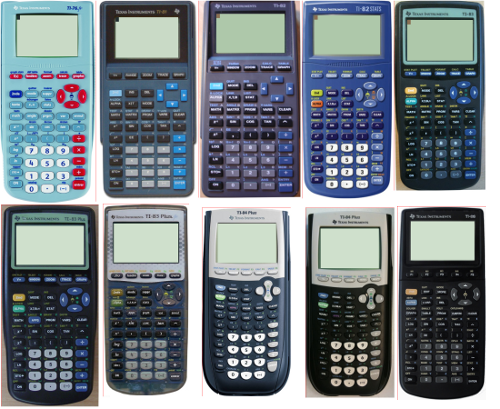
\includegraphics{pixs/diaporama_skin.png}}
\caption{The skins}
\end{figure}

\chapter{Installation}
\section{Generalities}
Before installing TilEm2, you should know that no ROM is included in this software.\newline
In order to use TilEm2, you must use your own rom (use TILP to get it).\newline

\section{Dependancies}
TilEm2 uses the following libraries :\newline
\begin{itemize}
\item	GTK+ 2.6 or higher (but 3.x not supported yet).
\item	libticalcs2.
\end{itemize}

\section{Install from sources}
Dowload the source from the trunk like this :\newline
svn co https://tilem.svn.sourceforge.net/svnroot/tilem\newline\newline

Then install gtk+ (e.g. for debian : sudo apt-get install libgtk2.0-dev).\newline
Then install libticalc2.\newline\newline

After that, simply use the configure script and the well know Linux install :\newline
./configure
make
sudo make install

Usually, icons will be copied into /usr/share/tilem2/\newline
Keybindings and configuration file will be installed into \$HOME/.config/tilem2\newline

Then you can launch TilEm2 with the command :\newline
tilem2 -r /path/to/rom\newline\newline

Or simply :\newline
tilem2\newline\newline

\section{First use}
If no rom is loaded, simply click right on the window and choose "Open Calculator...".\newline
The last used rom is automatically used for the next launch of TilEm2.\newline
You can save the current state of the calculator by using "Save Calculator".\newline

\chapter{Utilisation}
\section{Menu}
As TilEm1, the menu is a popup menu (right click).\newline
All you want to do need to use this menu.\newline
\begin{figure}[H]
\centering
\scalebox{1}{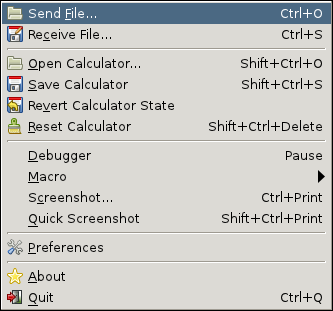
\includegraphics{pixs/popup.png}}
\caption{The right click menu}
\end{figure}
As you can see, there's all you need, no more, no less:\newline
\begin{itemize}
\item	Send File... : Load a file from your computer to TilEm2.
\item	Receive File : Launch a menu where you can store a variable from TilEm2 to your computer.
\item	Open Calculator... : Load a ROM.
\item	Save Calculator : Save the current state of the calculator (in a separate sav file)
\item	Revert Calculator : Revert the state of the calculator.
\item	Reset Calculator : Reset the calc of course.
\item	Debugger : Open the debugger window.
\item	Macro : Record, play, open or save a macro (a kind of script to do some actions automatically).
\item	Screenshot : Open the screenshot menu (static and animated screenshot).
\item	Quick Screenshot : Grab a screenshot and save it without prompting (that's why it's "quick").
\item	Preferences : Open the preference window.
\item	About : Open the about dialog (informations on the authors and more)
\item	Quit : Close TilEm2 properly
\end{itemize}

\section{Send File...}

\begin{figure}[H]
\centering
\scalebox{1}{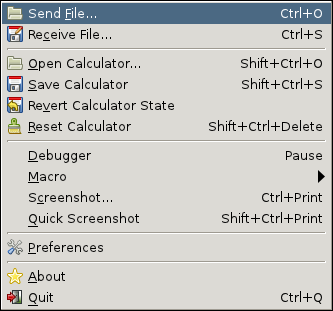
\includegraphics{pixs/send_file.png}}
\caption{The "Send File..." menu entry}
\end{figure}
This is one very important feature, because emulators are usually used to try some programs before really transferring it to real calc.\newline\newline
When you click on this menu entry, a file chooser dialog is opened and let you choose a file.\newline
\begin{figure}[H]
\centering
\scalebox{1}{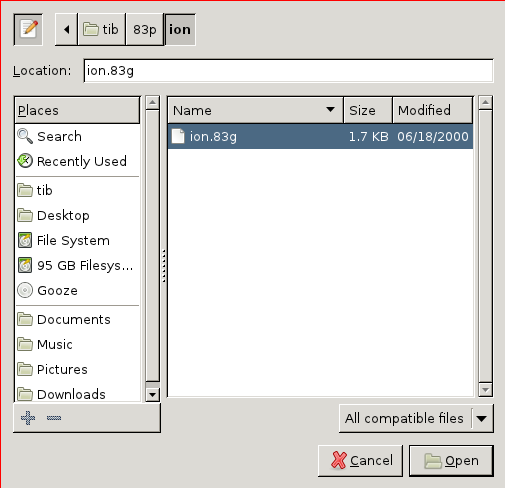
\includegraphics{pixs/send_file_chooser.png}}
\caption{The "Send File..." file chooser dialog}
\end{figure}
A lot of people don't know which file extension is associated with the emulated model...\newline
To help them, some patterns are used to do the selection.\newline
When you let "All compatible files", TilEm2 do the job for you, but you can choose "All files" if you know what you're doing (a file with an incorrect extension by example).\newline
\begin{figure}[H]
\centering
\scalebox{1}{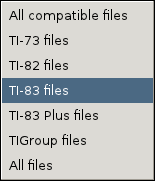
\includegraphics{pixs/send_file_chooser_pattern.png}}
\caption{The "Send File..." patterns}
\end{figure}

It could take some time to load a variable so a current progress bar is printed while loading to know what's happening.\newline

\begin{figure}[H]
\centering
\scalebox{0.5}{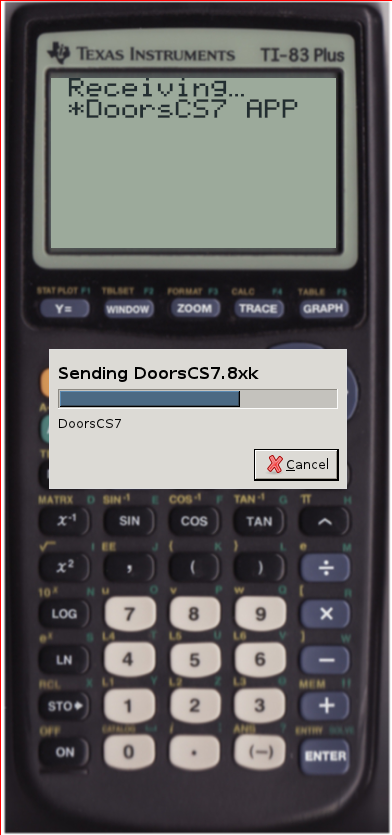
\includegraphics{pixs/send_file_loading.png}}
\caption{The "Senf File..." progress bar update}
\end{figure}

\section{Receive File...}
\begin{figure}[H]
\centering
\scalebox{0.8}{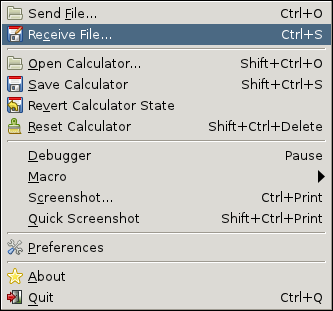
\includegraphics{pixs/receive_file.png}}
\caption{The "Receive File..." menu entry}
\end{figure}
When you click on "Receive File..." menu entry, TilEm2 firstly get the vars then prints it into a listview.\newline
\begin{figure}[H]
\centering
\scalebox{0.6}{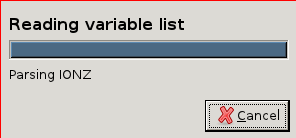
\includegraphics{pixs/receive_file_loading.png}}
\caption{The "Receive File..." get the variables}
\end{figure}
After the first launch, refresh is made only on request !\newline
If you click "Receive File..." then close the window, then create a program and click "Receive File..." you will not see your program.\newline
The variable list let you choose the stuff you want to backup.\newline
\begin{figure}[H]
\centering
\scalebox{0.8}{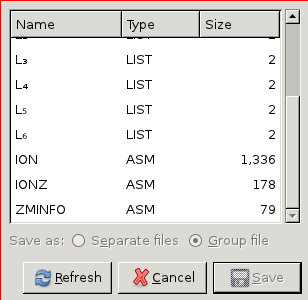
\includegraphics{pixs/receive_file_list.png}}
\caption{The "Receive File..." window}
\end{figure}
If more than one variable is selected, you can choose between two modes of backup :
"Separate files" or "Group file".\newline
If you choose separate, each file is saved as if you have saved one by one.\newline
\begin{figure}[H]
\centering
\scalebox{0.8}{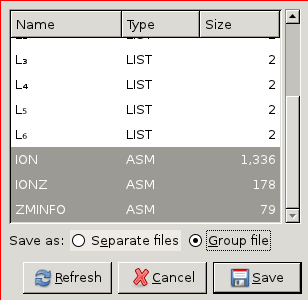
\includegraphics{pixs/receive_file_separate_or_grouped.png}}
\caption{The two modes of backup (multiple files only)}
\end{figure}
If you save grouped, a group file will be created on disk.\newline
When you finally click on "Save" button, a file save dialog is opened.\newline
Choose a directory and a name and click "Save".\newline
\begin{figure}[H]
\centering
\scalebox{0.8}{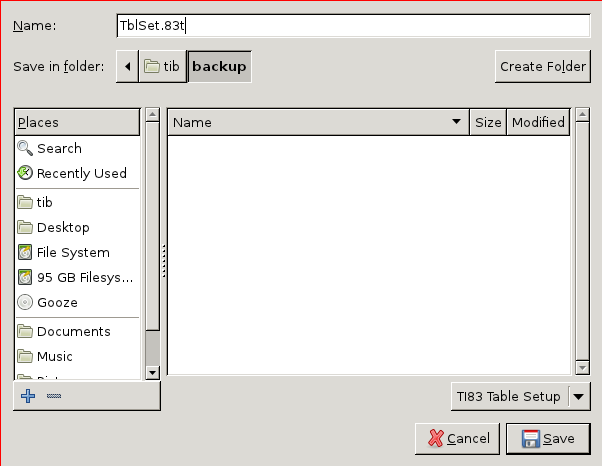
\includegraphics{pixs/receive_file_chooser.png}}
\caption{The "Receive File..." file save}
\end{figure}

\section{Open Calculator...}

\begin{figure}[H]
\centering
\scalebox{0.8}{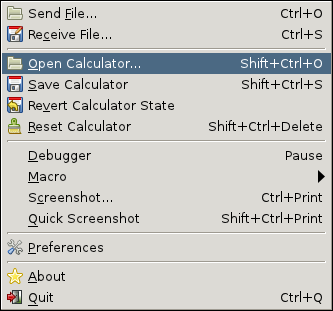
\includegraphics{pixs/open_rom.png}}
\caption{The "Open Calculator..." menu entry}
\end{figure}
When you click on "Open Calculator...", a file chooser dialog pop up and let you choose a rom to load.\newline
So in fact even if you already emulates a calculator, you can switch to another just by opening a new rom file.\newline
Another way to do that is to quit TilEm2 and restart it using another rom file (option -r).\newline

\begin{figure}[H]
\centering
\scalebox{0.8}{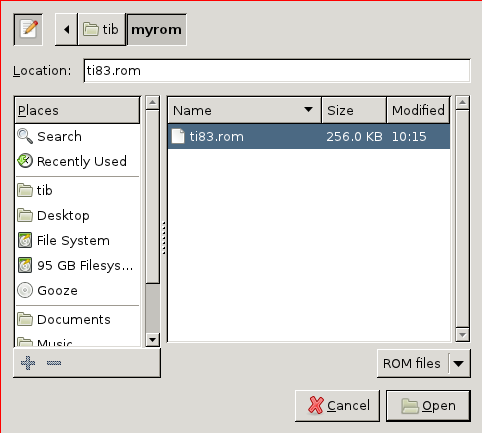
\includegraphics{pixs/open_rom_chooser.png}}
\caption{The "Open Calculator..." file chooser}
\end{figure}
Rom files usually finish by .rom as extension but you can use "All files" pattern if you have a rom with a odd extension.\newline
\begin{figure}[H]
\centering
\scalebox{0.8}{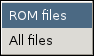
\includegraphics{pixs/open_rom_chooser_pattern.png}}
\caption{The file chooser patterns}
\end{figure}


\section{Save Calculator...}

\begin{figure}[H]
\centering
\scalebox{0.8}{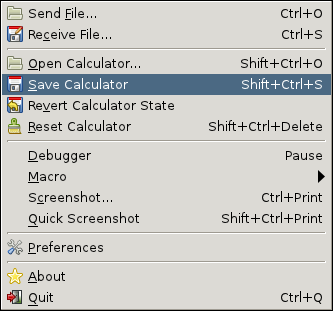
\includegraphics{pixs/save_calculator.png}}
\caption{The "Save Calculator" menu entry}
\end{figure}

This option just save the current state of the calculator in a .sav file.\newline
The file is created in the same directory as the rom file and with the same name.\newline
\section{Revert Calculator State}

\begin{figure}[H]
\centering
\scalebox{0.8}{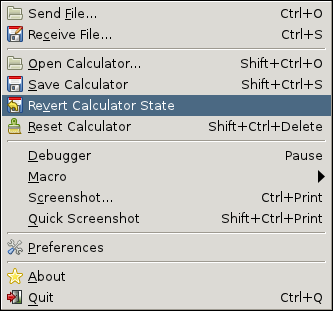
\includegraphics{pixs/revert_calculator.png}}
\caption{The "Revert Calculator State" menu entry}
\end{figure}

No surprise, this option just revert the calculator state (if possible).\newline

\section{Reset Calculator}

\begin{figure}[H]
\centering
\scalebox{0.8}{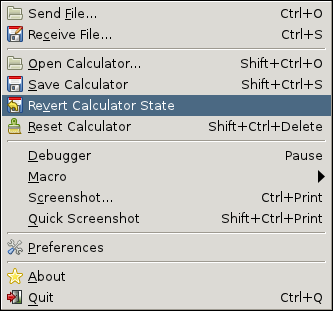
\includegraphics{pixs/revert_calculator.png}}
\caption{The "Reset Calculator" menu entry}
\end{figure}

Guess what does this option :)

\section{Debugger}

\begin{figure}[H]
\centering
\scalebox{0.8}{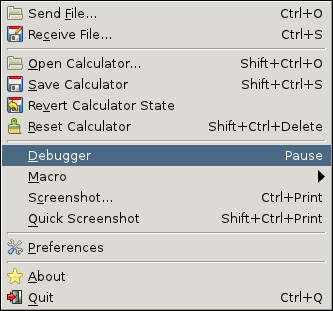
\includegraphics{pixs/debugger.png}}
\caption{The "Debugger" menu entry}
\end{figure}
When you click on this option, the debugger window will appear.\newline

\begin{figure}[H]
\centering
\scalebox{0.8}{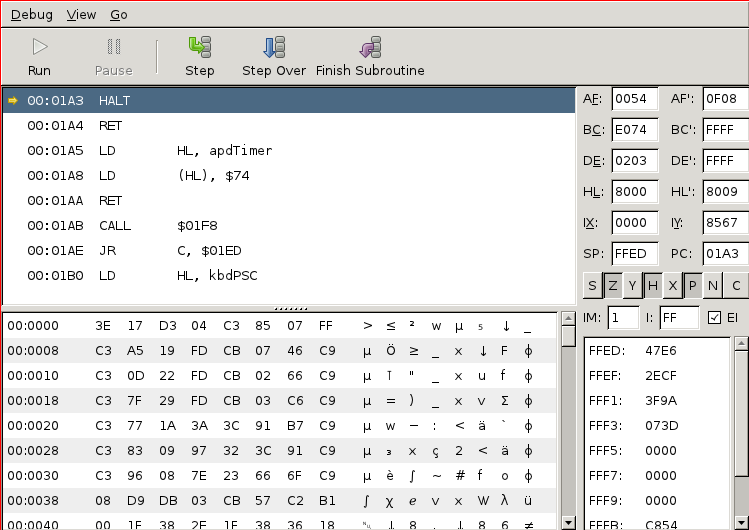
\includegraphics{pixs/debugger_dialog.png}}
\caption{A nice and powerful debugger}
\end{figure}
There's a lot of things to say about debugger.\newline
When you launch it, calculator is automatically paused.\newline
As you can see there are 5 big buttons : Run, Pause, Step, Step Over, Finish Subroutine.\newline
Step just execute one instruction.\newline
As you can see, all the instructions are not the same length, that's why it doesn't step one byte per one byte.\newline
Step over do the same job than step but do not follow call.\newline
Finish subroutine just do basically the same job but stop after a ret.\newline

Now just see what's the differents view of the debugger dialog.\newline
There's a big frame for disassembly view.\newline
In this frame, you can see the adress and the disassembly instruction.\newline
On right click, you can do some useful actions : Breakpoint here, Go to adress, go to PC.\newline
\begin{figure}[H]
\centering
\scalebox{0.8}{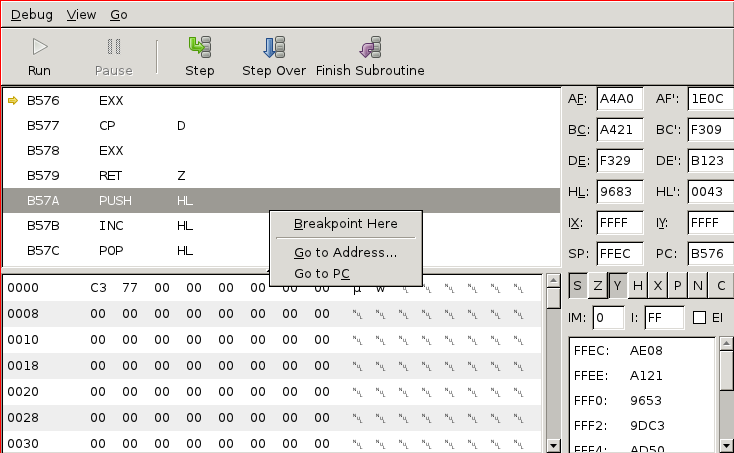
\includegraphics{pixs/debugger_disasm_popup.png}}
\caption{The right click menu on disasm view}
\end{figure}

There's 2 kind of adress notation for this view : Logical and Absolute.\newline 
You can switch it into the "View" menu.\newline

\begin{figure}[H]
\centering
\scalebox{0.8}{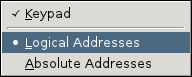
\includegraphics{pixs/debugger_logical.png}}
\caption{Switch between logical and absolute adresses}
\end{figure}
The second big frame is the memory view.\newline
For this view you can switch the adresses representation if you want.\newline
In this view you can see what your calculator contains.\newline
You can also edit the memory and change some values by your own.\newline
\begin{figure}[H]
\centering
\scalebox{0.8}{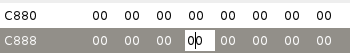
\includegraphics{pixs/debugger_memory_edit.png}}
\caption{Edit the memory}
\end{figure}
A third view represents the registers.\newline
You can edit them too.\newline
Below registers there is a bunch of toggle button to represent the flags (you can change it).\newline
Then Interruption Mode IM, I, and Enable Interrupt (checkbox).\newline
The finally the stack.\newline

At the top of the debugger window, you can see a menu "Debug".\newline
\begin{figure}[H]
\centering
\scalebox{0.8}{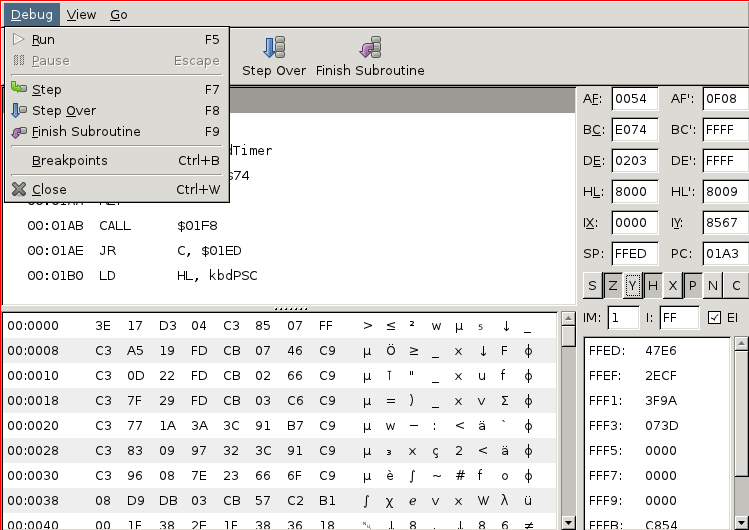
\includegraphics{pixs/debugger_debug.png}}
\caption{The "Debug" menu entry}
\end{figure}
The options are the same than buttons but there is a big news : breakpoints.\newline
Breakpoints are a big part of the life of a assembly developpers.\newline
This option opens the Breakpoint menu when you can "Add", "Remove", "Edit", "Clear" or some special action like "Break on invalid instructions" or "Break on undocumented instructions".\newline

\begin{figure}[H]
\centering
\scalebox{0.8}{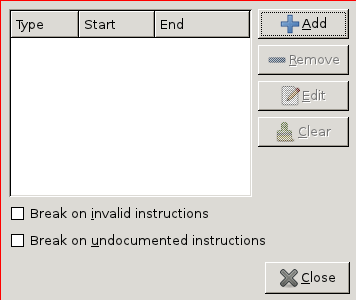
\includegraphics{pixs/debugger_breakpoint.png}}
\caption{The "Breakpoints" menu}
\end{figure}
The easiest way to add a breakpoint is to right click on the disasm view and click on "Breakpoint here" but you can also set a breakpoint using its adress (logical or absolute).\newline
\begin{figure}[H]
\centering
\scalebox{0.8}{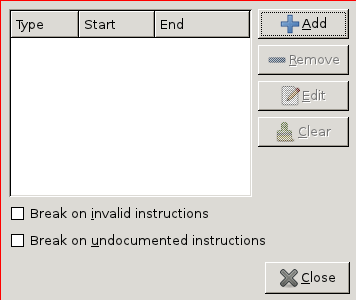
\includegraphics{pixs/debugger_breakpoint.png}}
\caption{Adding a breakpoint}
\end{figure}

The "Go" menu basically provide and easy way to navigate into the disasm view and th e stack.\newline
\begin{figure}[H]
\centering
\scalebox{0.8}{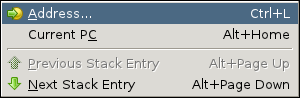
\includegraphics{pixs/debugger_go.png}}
\caption{The "Go" menu entry}
\end{figure}

Now I must talk about a nice tool called Keypad (into View menu).\newline
\begin{figure}[H]
\centering
\scalebox{0.8}{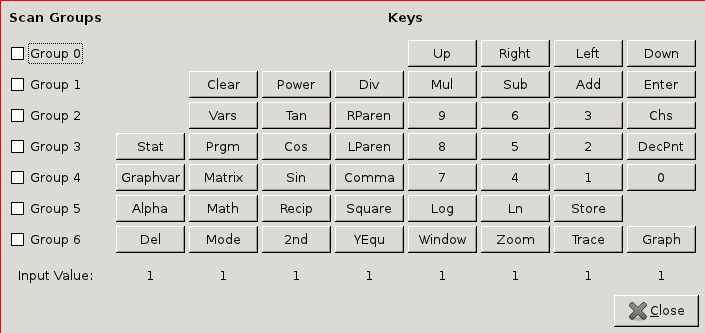
\includegraphics{pixs/debugger_keypad.png}}
\caption{The keypad}
\end{figure}

\section{Macro}

Macros are an easy way to simulates key press, file loading, reset automatically.\newline
It means that you could record a macro then click on some keys, then stop.\newline
If you play it, tilem will press the same keys for you.\newline
Have you never think too lazy to press always "2nd catalog asm(" each time you want to test your new asm production.\newline
Simply use a macro to load and launch your program automatically !\newline
\begin{figure}[H]
\centering
\scalebox{0.8}{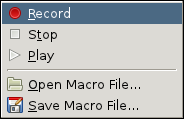
\includegraphics{pixs/macro.png}}
\caption{The "Macro" submenu}
\end{figure}
About the options, you can play an already loaded macro or a macro you just have recorded.\newline
You can also open a macro and save the current macro (which one you just have recorded).\newline

\section{Screenshot...}
\begin{figure}[H]
\centering
\scalebox{0.8}{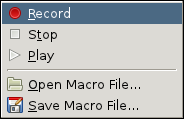
\includegraphics{pixs/macro.png}}
\caption{The "Screenshot..." submenu}
\end{figure}
By clicking on this option, you launch a screenshot dialog.\newline

\begin{figure}[H]
\centering
\scalebox{0.8}{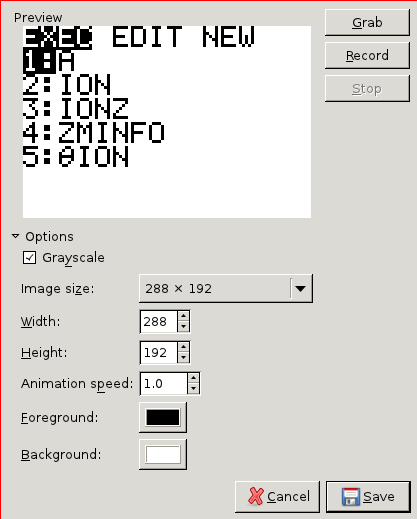
\includegraphics{pixs/screenshot_dialog.png}}
\caption{The screenshot dialog}
\end{figure}
You can grab static screenshot (multiple format) or animated screenshot (will be saved as gif).\newline
As you can see TilEm2 has a lot of screenshot configuration.\newline
So you can change the size, change the foreground and background colors.\newline
Use or not grayscale.\newline

\section{Preferences}

This is where you can set the skin (or disable using it) and some important other stuff.\newline
\begin{figure}[H]
\centering
\scalebox{0.8}{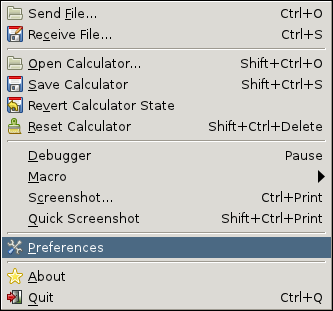
\includegraphics{pixs/preferences.png}}
\caption{The "Preferences" menu entry}
\end{figure}

You can limit speed or not.\newline
Emulate grayscale (if you don't know just let it checked by default).\newline
Use smooth scrolling.\newline
\begin{figure}[H]
\centering
\scalebox{0.8}{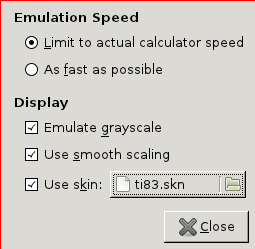
\includegraphics{pixs/preferences_dialog.png}}
\caption{The preferences dialog}
\end{figure}
And an important user friendly feature...\newline
Set skin !\newline
When you click on the button, a file choose will popup and lt you choose the skin.\newline
\begin{figure}[H]
\centering
\scalebox{0.8}{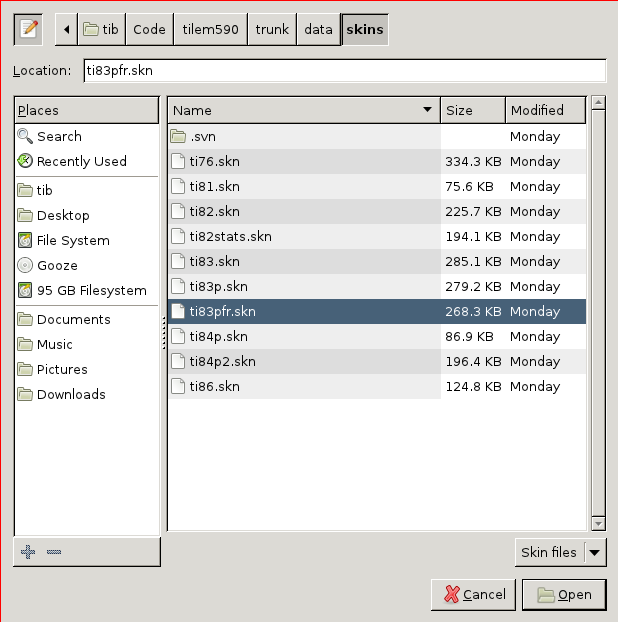
\includegraphics{pixs/skin_file_chooser.png}}
\caption{The skin file chooser}
\end{figure}

\section{About}

\begin{figure}[H]
\centering
\scalebox{0.8}{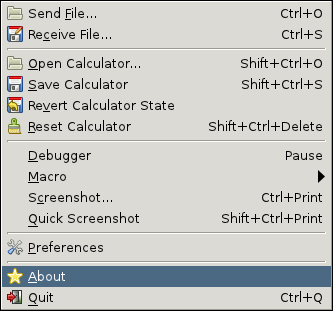
\includegraphics{pixs/about.png}}
\caption{The "About" menu entry}
\end{figure}
No more than an about dialog :)\newline

\begin{figure}[H]
\centering
\scalebox{0.8}{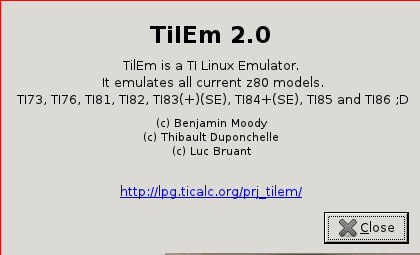
\includegraphics{pixs/about_dialog.png}}
\caption{The about dialog}
\end{figure}

\section{Quit}

\begin{figure}[H]
\centering
\scalebox{0.8}{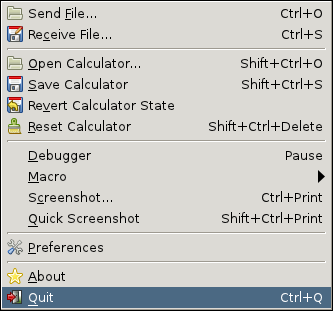
\includegraphics{pixs/quit.png}}
\caption{The "Quit" menu entry}
\end{figure}
Bye Bye ;)

\chapter{Command line usage}
TilEm2 is basically made for Linux and command line is our first love :)\newline
Here the options at launch.\newline
\begin{itemize}
\item  -r, --rom=FILE            The rom file to run
\item  -k, --skin=FILE           The skin file to use
\item  -m, --model=NAME          The model to use
\item  -f, --file=FILE           The file to load
\item  -s, --state-file=FILE     The state-file to use
\item  -l, --without-skin        Start in skinless mode
\item  --reset                   Reset the calc at startup
\item  --get-var=FILE            Get a var at startup
\item  -p, --play-macro=FILE     Run this macro at startup
\item  -d, --debug               Launch debugger
\end{itemize}

You should usually use something like : \newline
tilem2 -r /path/to/my/rom\newline\newline

But as you can see you can specify the skin with -k.\newline
If you usually use more than one model, you can try -m and it will load the rom associated with this model (if you already start a rom from this model).\newline
You can specify a different save state (by default it uses the one which is called as the rom file).\newline
You can start skinless.\newline
You can load a file and even launch a macro at startup (in this case loading a file is done before macro playing).\newline
You can reset too, get a var (if possible) and launch debugger.\newline
Something is missing?\newline


\chapter{Configuration files}
\section{General configuration}
\section{Keybindings}


\end{document}
